% =====================================================================
% agrupamiento.tex
% Responsabilidad única: presentar los perfiles de muestra (análisis
% elegido) y los segmentos de clientes (complementario), la diferencia de
% silueta entre el cribado y la etapa 06 y por qué se mantuvo la selección.
% Cifras: macros Agr*; tablas tabla_agr_*; figuras 06_*.
% =====================================================================
\section{Agrupamiento: perfiles de muestra y segmentos de clientes}
\label{sec:agrupamiento}

El agrupamiento no tiene una respuesta correcta contra la cual medirse, así
que se usa de forma descriptiva y con dos controles de honestidad, el
estadístico de Hopkins (tendencia a agruparse, 0.5 para datos sin estructura)
y la estabilidad de los grupos al cambiar la semilla. Se estudian dos
análisis, el elegido por la regla, \codigo{\AgrSeleccionado}
(\AgrSelFilas{} muestras aceptadas, \AgrSelVariables{} variables, de las
cuales \AgrSelConLog{} con $\log(1+x)$), y el complementario,
\codigo{\AgrComplementario} (\AgrCompFilas{} clientes, \AgrCompVariables{}
variables agregadas).

\paragraph{Escalado.} Sin escalar, la variable \AgrSelDominante{} aporta el
\AgrSelDominantePct{}\,\% de la varianza de los perfiles de muestra (y la
\AgrCompDominante{} el \AgrCompDominantePct{}\,\% en los segmentos), de forma
que K-means agruparía por una sola variable; el acuerdo (ARI) entre la
solución sin escalar y la escalada es de \AgrSelARISinEscalar{}, así que el
escalado no es un detalle, cambia por completo los grupos.

\subsection{Perfiles de muestra}

Con la matriz escalada (Hopkins de \AgrSelHopkins{}) se exploró K-means con
$k$ de \AgrKMin{} a \AgrKMax{}, con siluetas entre \AgrSelSiluetaMin{} y
\AgrSelSiluetaMax{}, y se eligió $k=\AgrSelK$ (silueta de
\AgrSelSilueta{}). La silueta es baja, es decir, las fronteras entre grupos
son difusas, pero la solución es estable, con un ARI entre
\AgrSelEstabilidadMin{} y \AgrSelEstabilidadMax{} frente a
\AgrSemillasEstabilidad{} semillas adicionales. La
Tabla~\ref{tab:agr-perfiles} nombra cada grupo por las variables que se
apartan más de \AgrUmbralNombre{} desviaciones estándar de la media.

\begin{table}[!htbp]
\centering
\tablaancha{agr_sel_grupos}
\caption{Perfiles de muestra de K-means, nombrados por las variables que los
distinguen (en desviaciones estándar, DE, respecto a la media general).}
\label{tab:agr-perfiles}
\end{table}

DBSCAN, con $\varepsilon=\AgrSelDBEps$ y \codigo{min\_samples} de
\AgrSelDBMinMuestras{} (\AgrSelDBConGrupos{} de las
\AgrSelDBCombinaciones{} combinaciones de la rejilla dieron dos o más grupos),
encuentra \AgrSelDBGrupos{} grupos densos con un \AgrSelDBRuidoPct{}\,\% de
ruido y una silueta sin ruido de \AgrSelDBSilueta{}, y su acuerdo con K-means
es bajo (ARI de \AgrSelARIKmDb{}). La Figura~\ref{fig:agr-pca} muestra por
qué, ya que K-means parte una nube continua en regiones, mientras que DBSCAN
solo separa la zona densa aislada, que coincide con el perfil de plazo
prometido largo.

\begin{figure}[!htbp]
\centering
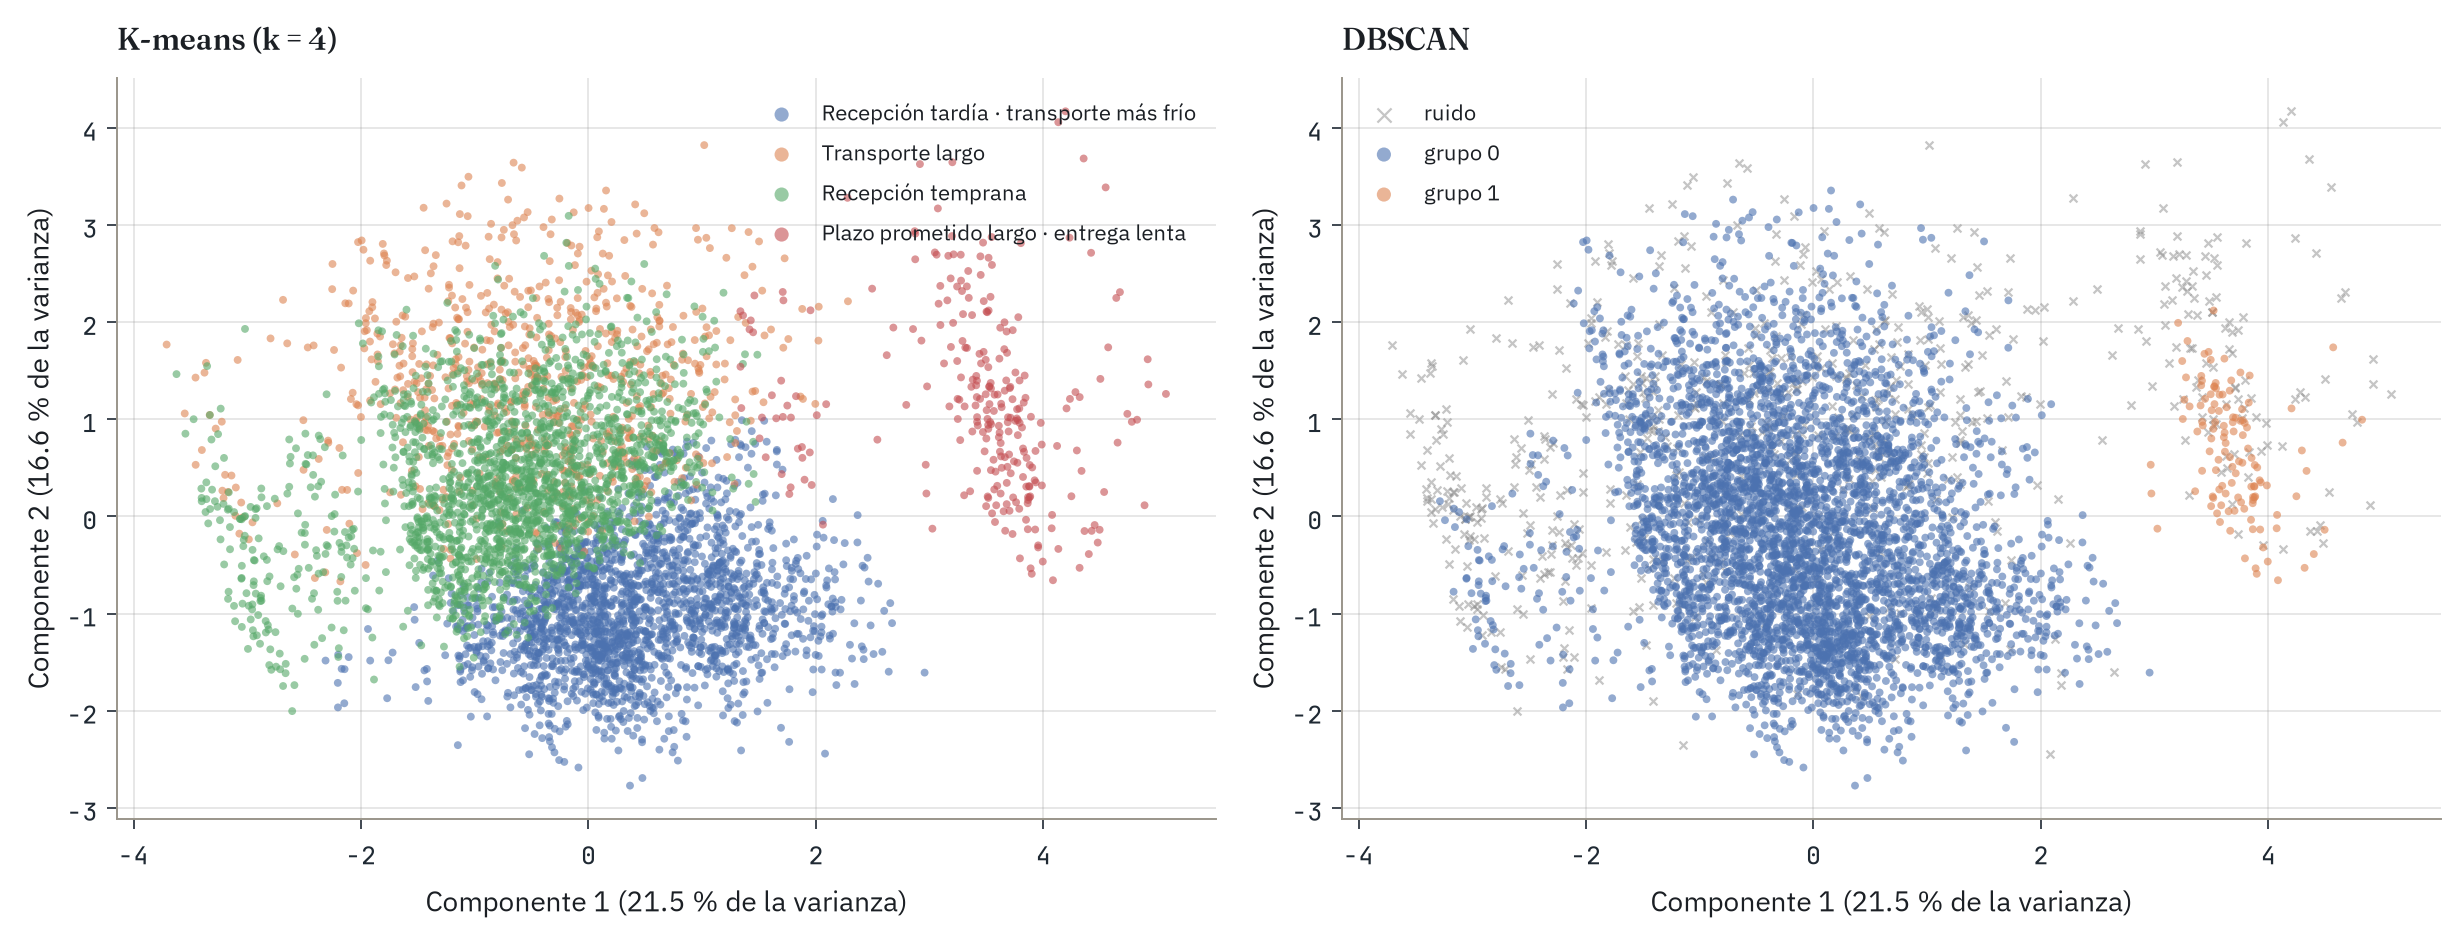
\includegraphics[width=0.85\textwidth]{06_perfiles_muestra_pca.png}
\caption{Perfiles de muestra en las dos primeras componentes principales
(\AgrSelPCAVarianzaPct{}\,\% de la varianza): K-means (izquierda) y DBSCAN
(derecha, ruido en gris). La única región bien separada es la de la derecha;
el resto es una nube continua que K-means corta en franjas.}
\label{fig:agr-pca}
\end{figure}

\subsection{Segmentos de clientes}

En los clientes (Hopkins de \AgrCompHopkins{}) se eligió $k=\AgrCompK$, con
una silueta de \AgrCompSilueta{} y una estabilidad entre
\AgrCompEstabilidadMin{} y \AgrCompEstabilidadMax{}. El segmento más grande
en volumen, «\AgrCompSegmentoMayor», reúne el
\AgrCompSegmentoMayorClientesPct{}\,\% de los clientes pero el
\AgrCompSegmentoMayorMuestrasPct{}\,\% de las muestras, y el segmento de más
no conformidad es también el de más entregas tardías
(Figura~\ref{fig:agr-segmentos}), lo que lo
hace el candidato natural para un seguimiento comercial y de calidad. En este
análisis DBSCAN no encontró dos grupos con ninguna combinación
(\AgrCompDBConGrupos{} de \AgrCompDBCombinaciones{}), así que se usa como
detector de atípicos ($\varepsilon=\AgrCompDBEps$, \AgrCompDBRuidoPct{}\,\% de
clientes marcados como ruido).

\begin{figure}[!htbp]
\centering
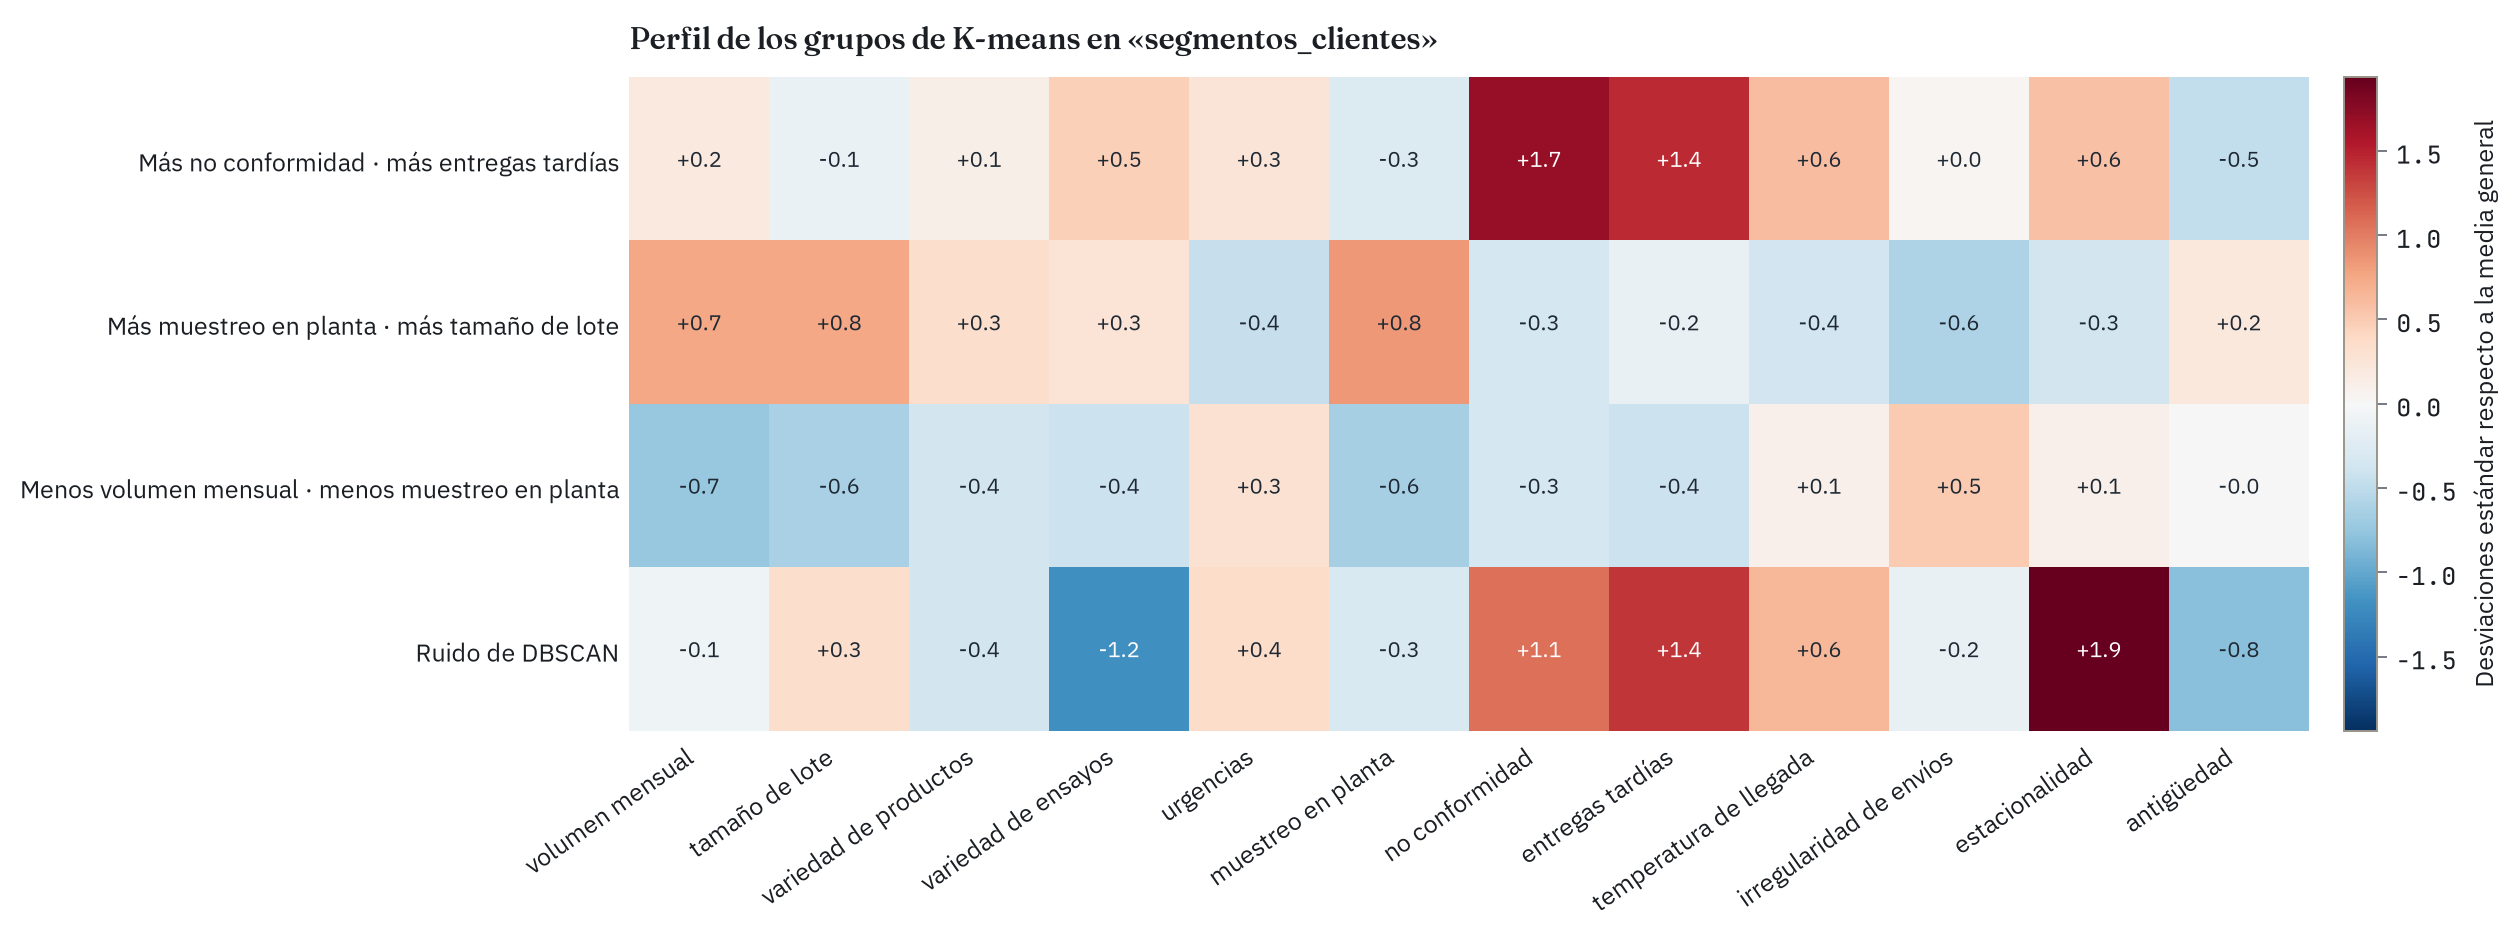
\includegraphics[width=0.9\textwidth]{06_segmentos_clientes_perfiles.png}
\caption{Perfil de los segmentos de clientes (desviaciones estándar respecto a
la media general). La fila inferior son los clientes que DBSCAN marca como
ruido: comparten la no conformidad y las entregas tardías altas del primer
segmento, pero con una estacionalidad mucho más marcada.}
\label{fig:agr-segmentos}
\end{figure}

\subsection{Silueta del cribado frente a la etapa 06}
\label{sec:silueta}

La silueta de los perfiles de muestra cae de \AgrSiluetaCribado{} en el
cribado a \AgrSelSilueta{} en la etapa~06, muy por encima de la diferencia
de \AgrToleranciaSilueta{} a partir de la cual el procedimiento la discute, y la
etapa~06 separa sus dos causas (Tabla~\ref{tab:agr-silueta}). El cambio de
filas (entrenamiento frente a todo el desarrollo) mueve la silueta en
\AgrEfectoFilas{} (\AgrSiluetaSinLog{} sin $\log(1+x)$), mientras que la
transformación $\log(1+x)$ antes de escalar la mueve en \AgrEfectoLog{}, de
forma que casi toda la caída se debe al preprocesamiento; una explicación
plausible (no verificada por separado) es que, sin el logaritmo, las colas
largas de unas pocas variables separan dos grupos con facilidad, y con él esa
separación desaparece.

\begin{table}[!htbp]
\centering
\tablaancha{agr_silueta_cribado}
\caption{Silueta y puntaje de la regla con el preprocesamiento del cribado y
con el de la etapa 06, para los dos análisis de agrupamiento.}
\label{tab:agr-silueta}
\end{table}

Con las siluetas de la etapa~06, el puntaje de la regla sería de
\AgrPuntajeSelEtapa{} para el análisis elegido y de \AgrPuntajeCompEtapa{}
para el complementario, es decir, el complementario habría ganado
(\AgrComplementarioSupera{}). Aun así se mantuvo la selección, porque la regla
se fijó antes de ver los resultados y cambiarla después equivaldría a elegir
a posteriori; en su lugar se reportan los dos análisis completos y
la discrepancia queda registrada como una lección para el cribado, que debe
usar el mismo preprocesamiento que el estudio a fondo.

\paragraph{Auditoría con la verdad de la simulación.} Solo con datos
simulados se puede comparar con los \AgrAudSegmentosLatentes{} segmentos
latentes del generador: en los \AgrAudClientes{} clientes auditados, el ARI
es de \AgrAudARIKmeans{} para K-means y de \AgrAudARIDbscan{} para DBSCAN, con
una pureza de \AgrAudPureza{}. Los segmentos recuperan solo en parte la
estructura latente, lo que es coherente con que el generador hace que los
segmentos se solapen a propósito.
